
 \begin{figure}[t]
	\centering
	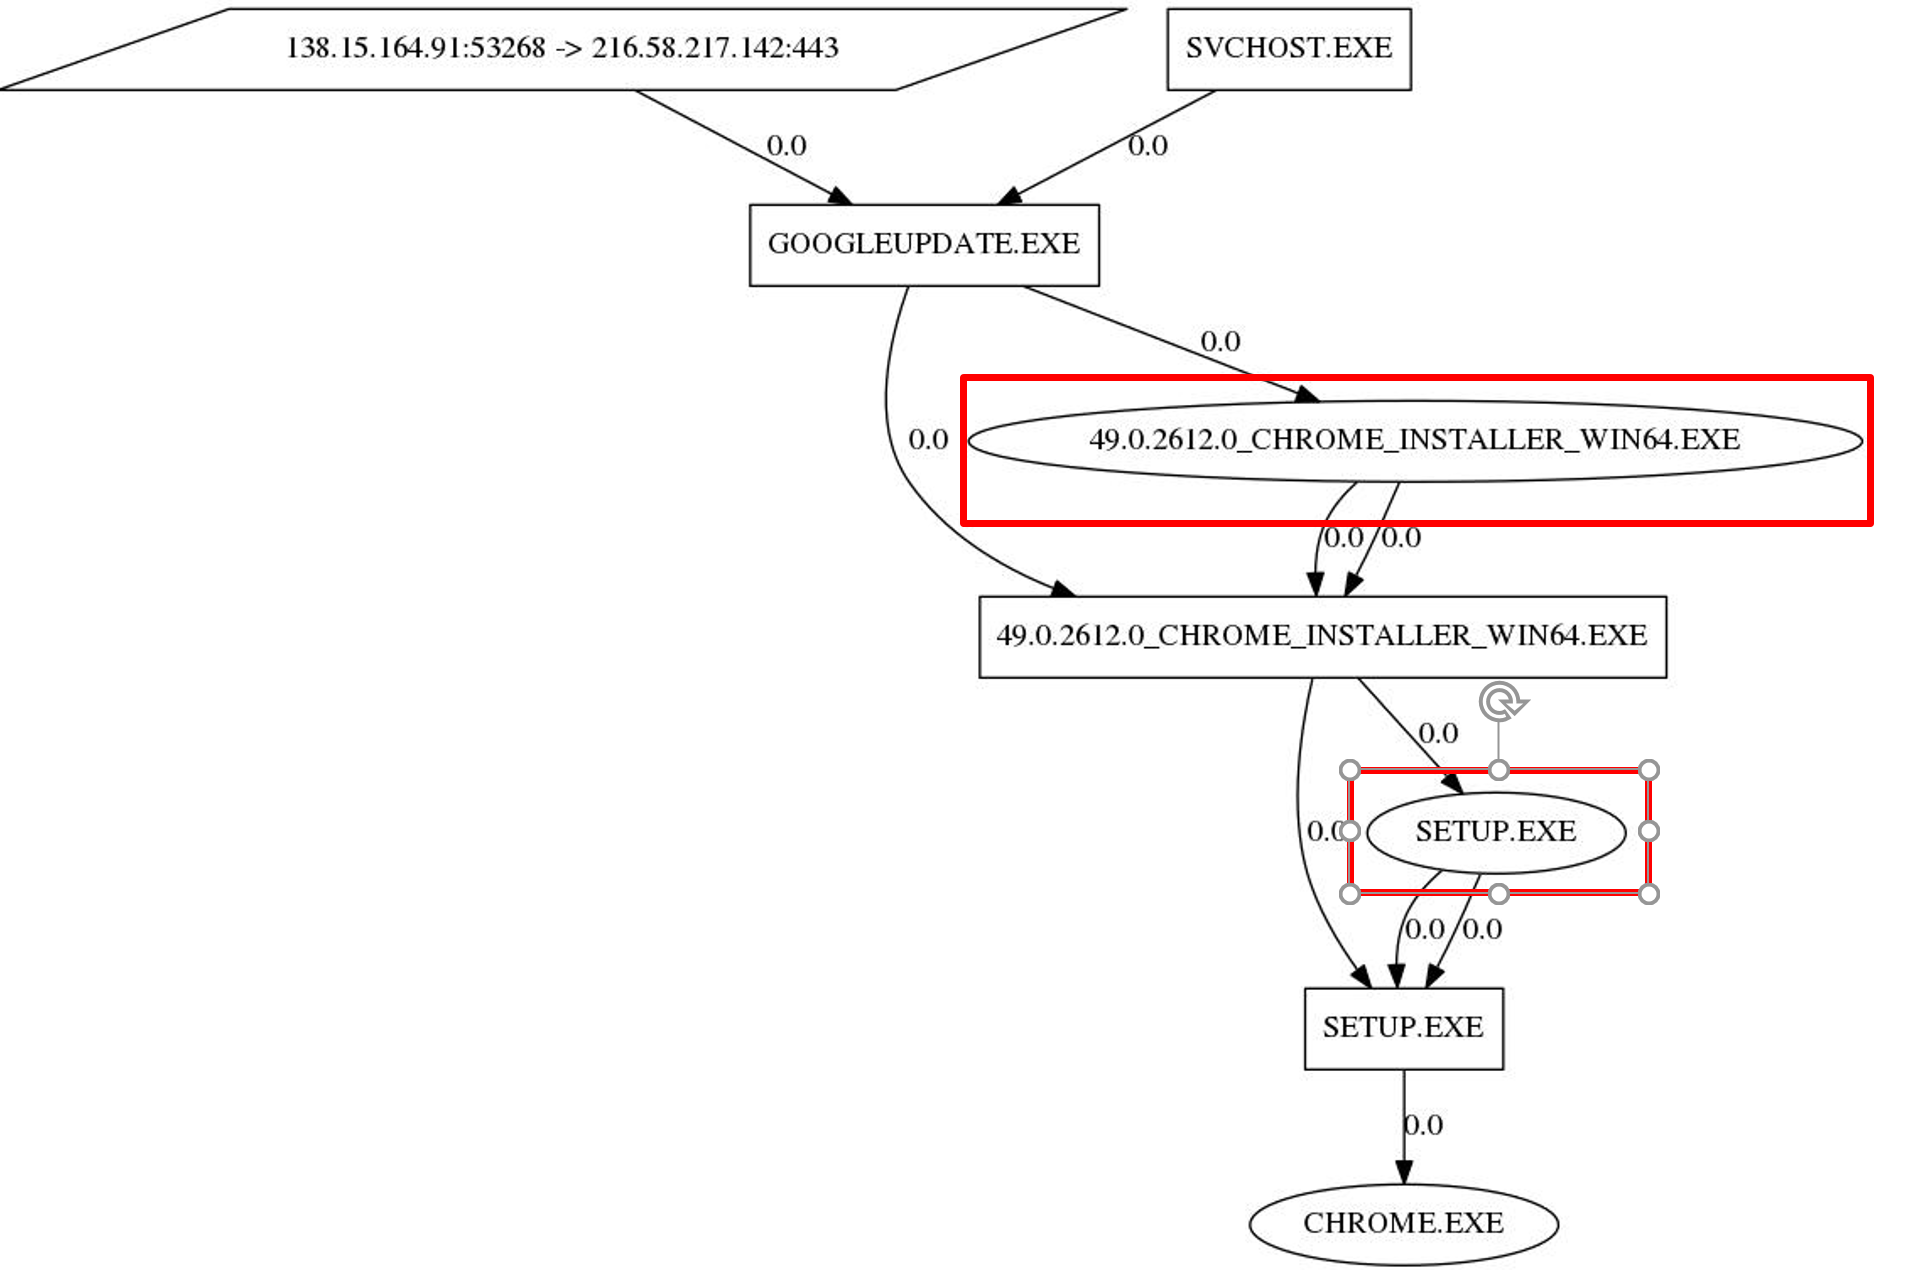
\includegraphics[width=0.5\textwidth]{testSample.png}
	\caption{Test sample}
	\label{fig:splitsample}
\end{figure} 

\section{Preliminary Result}
%\begin{figure*}[htp] 
%	\centering
%	\subfloat[original graph]{%
%		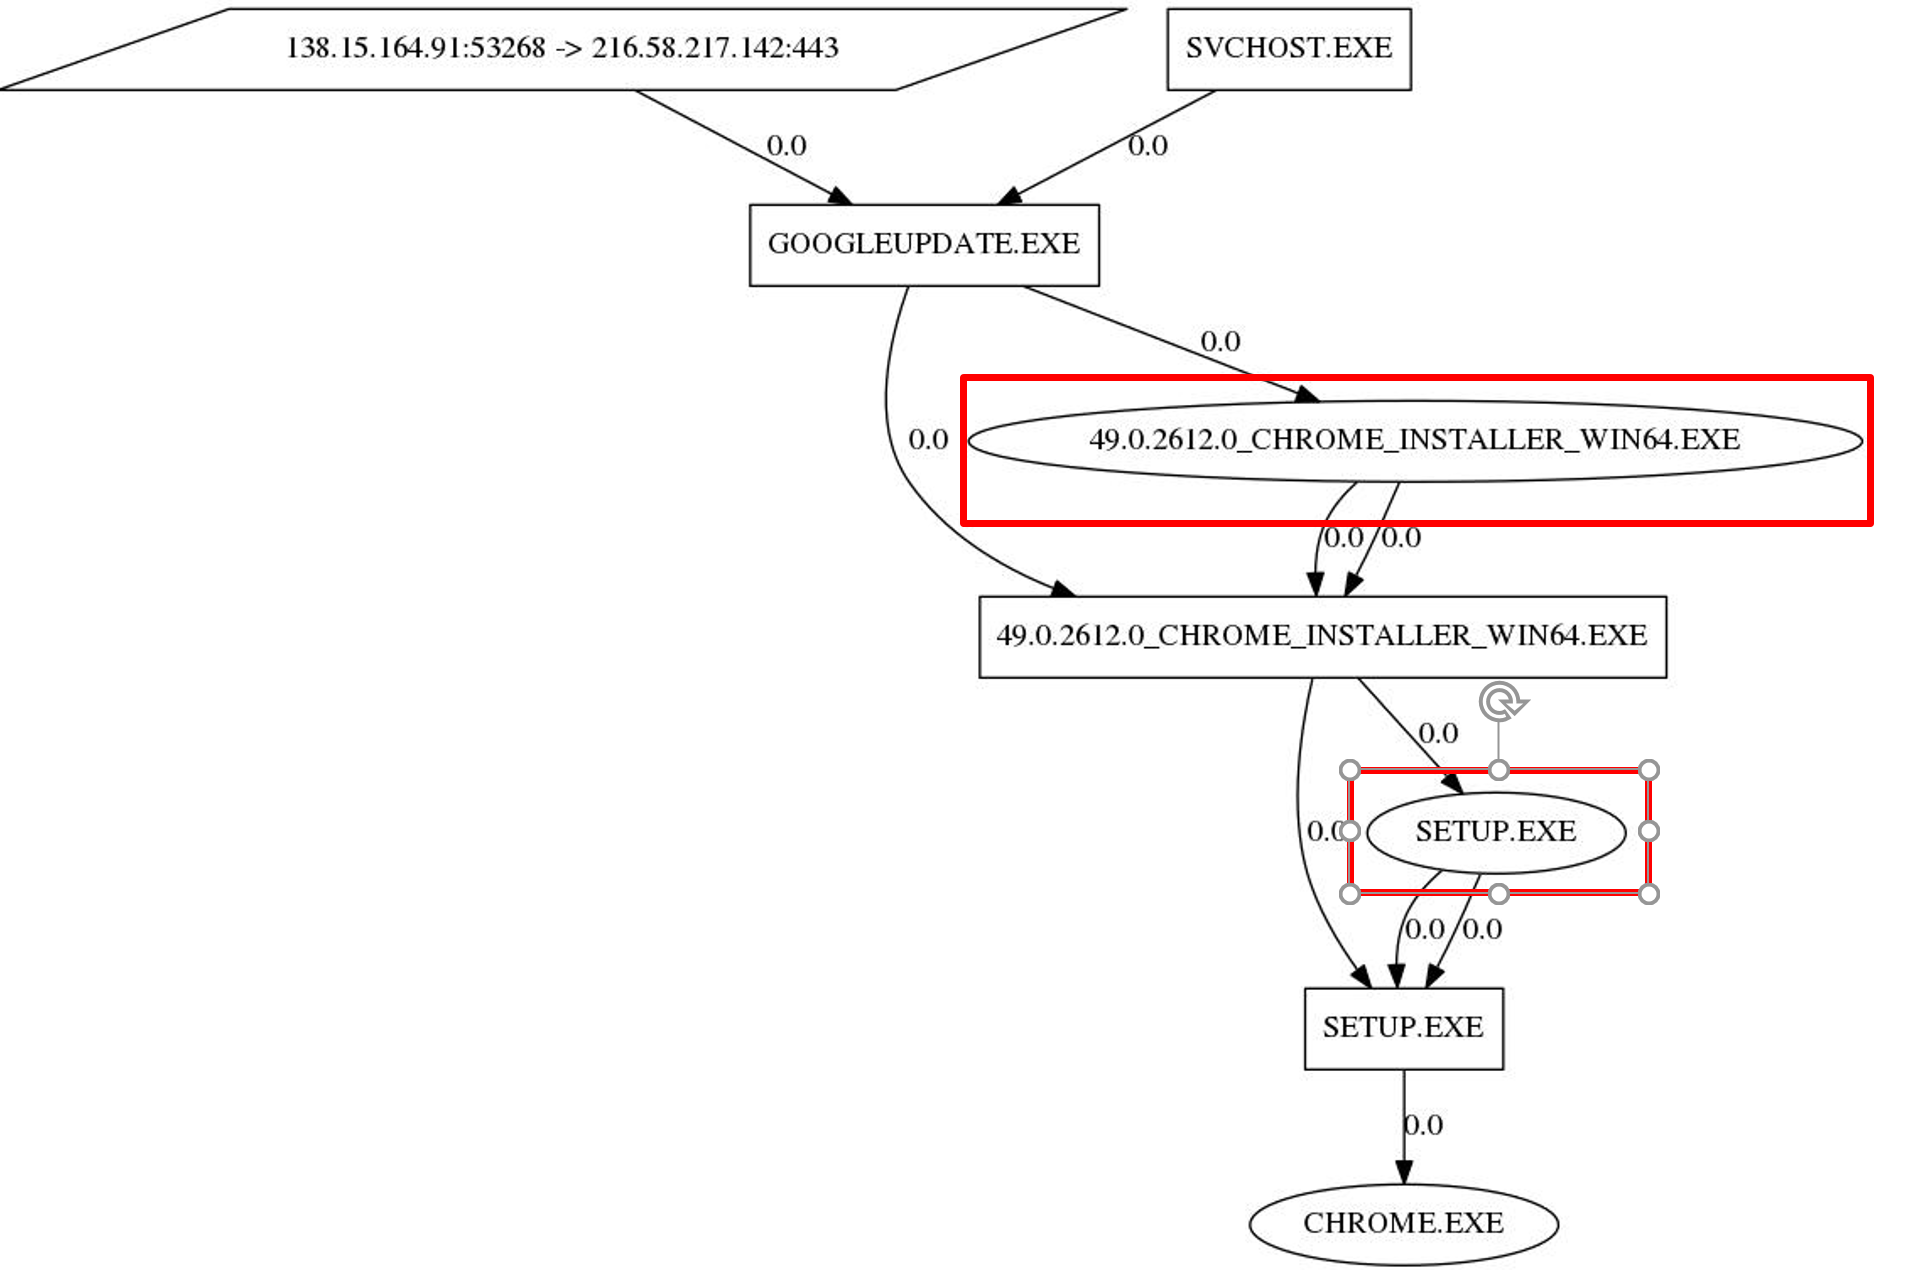
\includegraphics[width=0.5\linewidth,height=5cm]{testSample.png}%
%		\label{fig:a}%
%	}%
%	\hfill%
%	\subfloat[after splitting]{%
%		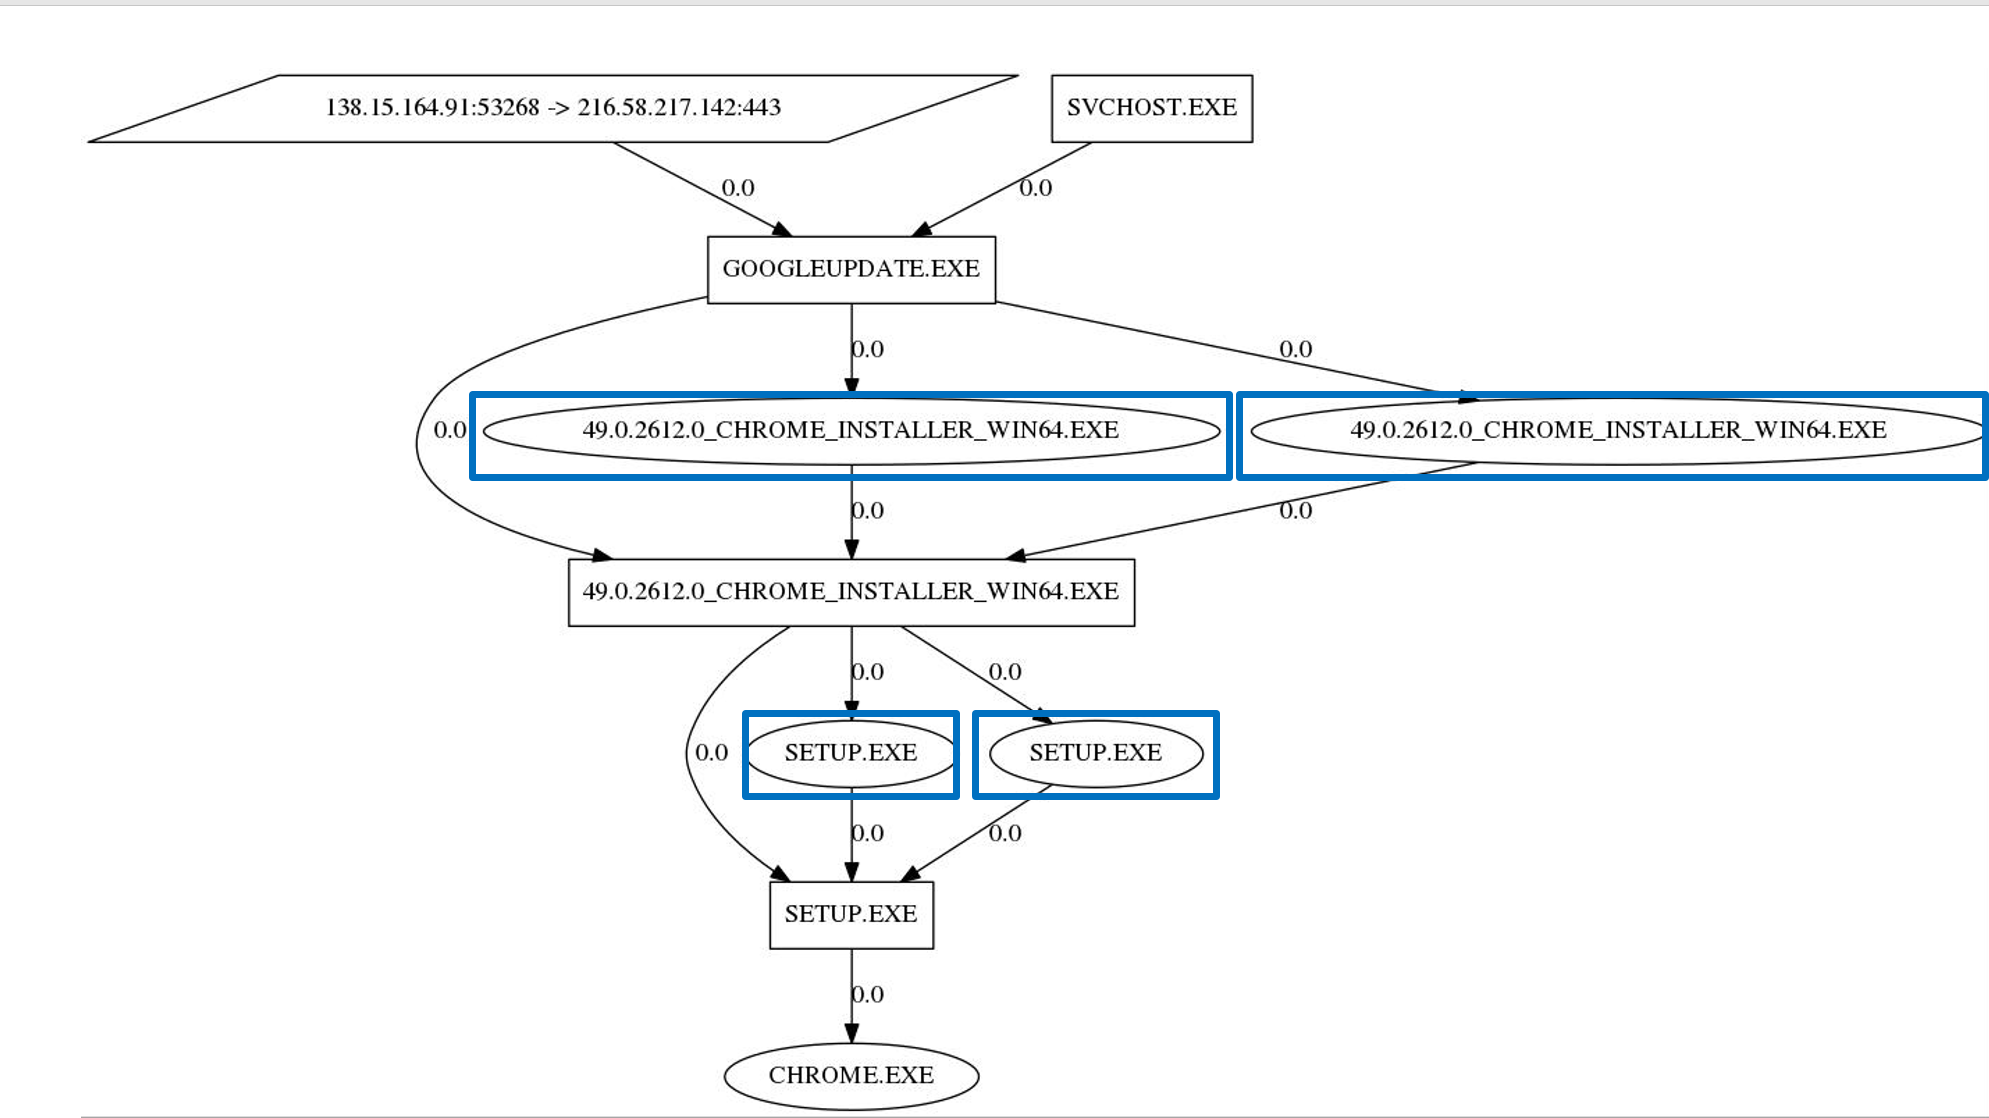
\includegraphics[width=0.5\linewidth,height=5cm]{sampleResult.png}%
%		\label{fig:b}%
%	}%
%	\caption{The test sample of Graph Split}
%	\label{fig:sampleResult}
%\end{figure*}

In this part, we will show preliminary results up until graph split. The first table show our method's performance on the system monitoring data. The first column show the test case is that user use Linux command: \textit{apt get} to install some applications. This operation is quite common in different environment. The second column is the log file size. We use the vertex and edge number to evaluate the size of the dependency graph. It is very obvious that our method reduce the number of vertex and edge in the dependency graph.  It reduce the burden for further calculation. We also already test out GraphSplit on a small sample from the real-world scenario. Figure~\ref{fig:splitsample} and Figure~\ref{fig:splitresult} are the sample results of \emph{GraphSplit}. The vertexes in the red square has multiple edges pointing to the same object, so this one need to be split. The vertex in the blue square is vertexes generated by \emph{Graphsplit} algorithm. In the next step, we will gather the aduiting data in a longer time and test its performance and overhead. 
%\begin{table*}
%	\centering
%	\caption{The size of log file and dependency graph}
%	\begin{tabular}{ |l|c|c|c|c|c|c|r| }{\textwidth}
%		\hline
%		apt-get Install unrar & log file size & vertex number $(origina)$ & edge number $(Orignal)$ & vertex number$(Backtracking)$ & edge number$(Backtracking)$ & vertex number $(CPR)$ & edge number$(CPR)$\\
%		\hline
%	\end{tabular}
%\end{table*}



\begin{figure}[t]
	\centering
	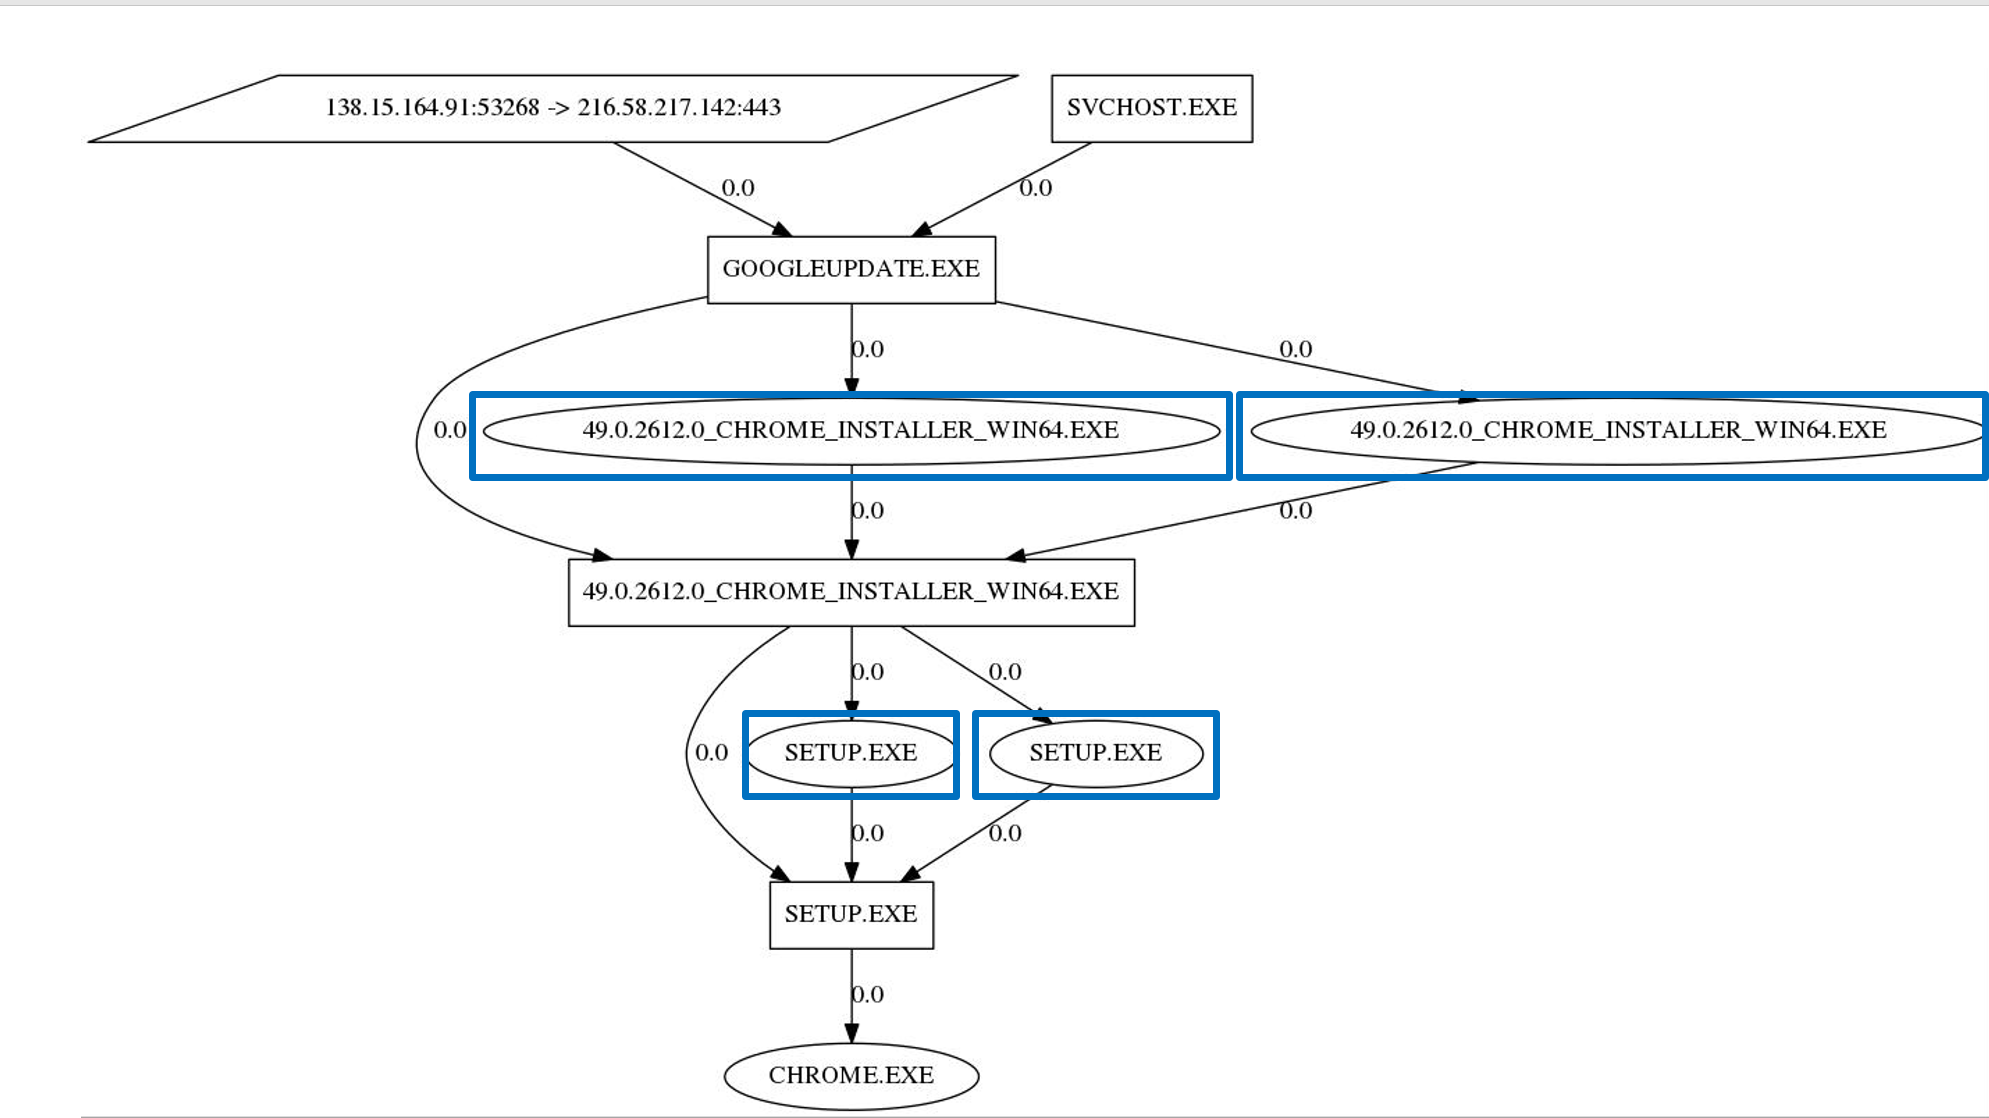
\includegraphics[width=0.5\textwidth]{sampleResult.png}
	\caption{GraphSplit Result}
	\label{fig:splitresult}
\end{figure}
\vspace{2cm}
%\begin{figure}[!htbp]
%	\begin{minipage}[t][0.8\textheight]{0.5\textwidth}
%		\centering
%		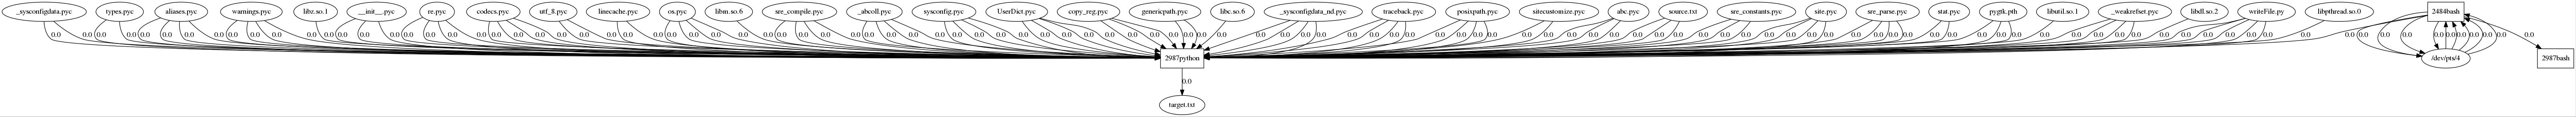
\includegraphics[align=c, width=\textheight,angle=90]{fileBack.jpg}
%		\hspace{0.1\textwidth}
%		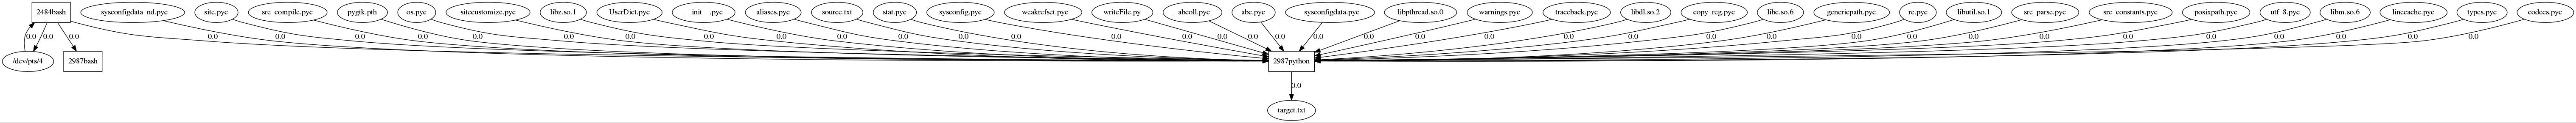
\includegraphics[align=c, width=\textheight,angle=90]{fileCPR.jpg}
%	\end{minipage}
%	\caption{Backtracking And Causality Preserve Reduction Result}
%	\label{fig:backandCPR}
%\end{figure}



